%
% buchcover.tex -- Cover für das Buch Numerik
%
% (c) 2018 Prof Dr Andreas Müller, Hochschule Rapperswil
%
\documentclass[11pt]{standalone}
\usepackage{tikz}
\usepackage{times}
\usepackage{geometry}
\usepackage{german}
\usepackage[utf8]{inputenc}
\usepackage[T1]{fontenc}
\usepackage{times}
\usepackage{amsmath,amscd}
\usepackage{amssymb}
\usepackage{amsfonts}
\usepackage{txfonts}
\usepackage{ifthen}
\usepackage{qrcode}
\usetikzlibrary{math}

\begin{document}
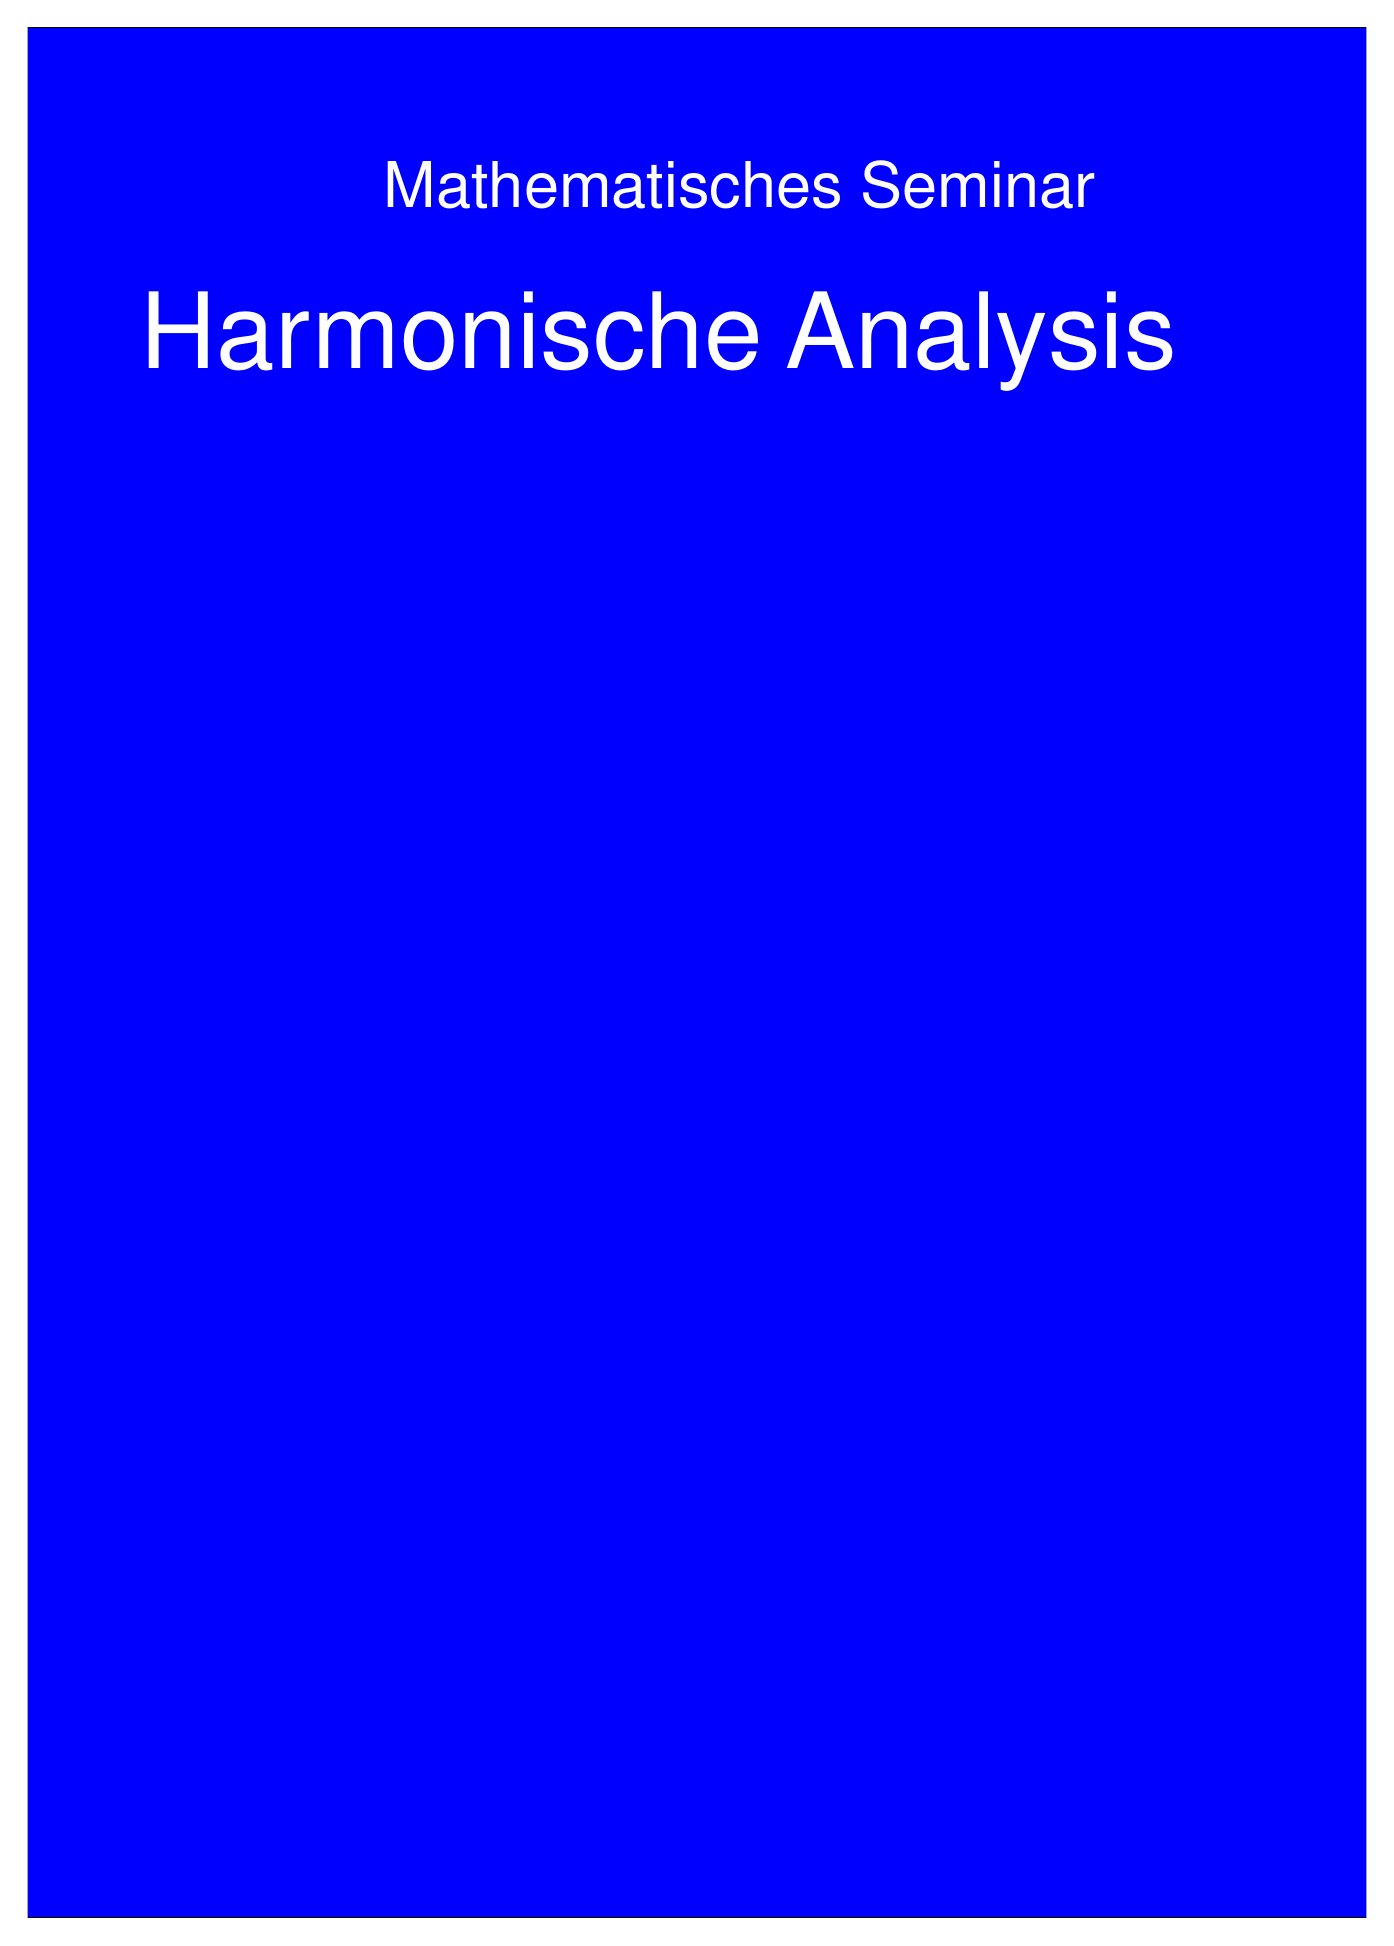
\begin{tikzpicture}[>=latex,scale=1]

\def\bogenbreite{17.0}
\def\bogenhoehe{24.0}

\clip (0,0) rectangle ({\bogenbreite},{\bogenhoehe});

\draw[fill=blue] (0,0) rectangle ({\bogenbreite},{\bogenhoehe});

%\begin{scope}
%\node at ({5},2.0) {\includegraphics[width=42cm]{../buch/chapters/090-pde/membran/membran.png}};
%\node at (-6,9) {\includegraphics[width=8cm]{../buch/chapters/090-pde/kugel/spherical33.png}};
%\node at (3,9) {\includegraphics[width=8cm]{../buch/chapters/090-pde/kugel/spherical32.png}};
%\node at (9.5,9) {\includegraphics[width=8cm]{../buch/chapters/090-pde/kugel/spherical31.png}};
%\node at (15.7,9) {\includegraphics[width=8cm]{../buch/chapters/090-pde/kugel/spherical30.png}};
%\end{scope}

\node at (7.5,22)
	[color=white,scale=1]
	{\hbox to\hsize{\hfill%
	\sf \fontsize{24}{24}\selectfont Mathematisches Seminar}};

\node at (7.5,20)
	[color=white,scale=1]
	{\hbox to\hsize{\hfill%
	\sf \fontsize{40}{40}\selectfont Harmonische Analysis}};

%\node at (7.5,16)
%	[color=white,scale=1]
%	{\hbox to\hsize{\hfill%
%	\sf \fontsize{13}{5}\selectfont Andreas Müller}};

\end{tikzpicture}
\end{document}
